\documentclass[11pt]{article}
\fontfamily{times}
\usepackage{graphicx}
\usepackage{amsmath}
\usepackage{geometry}
\usepackage{subcaption}

\geometry{verbose,tmargin=30mm,bmargin=25mm,lmargin=25mm,rmargin=25mm}
\newcommand{\templatefigures}[1]
{\noindent
\begin{minipage}{2cm}
\begin{center}
%\linespread{1}
%\begin{figure}
  \centering
	\vspace{-1cm}
  
\includegraphics[height = 63px]{ISI2019only_with_date_small.pdf}\\
    %\label{matrix}
%\end{figure}
\end{center}
\end{minipage}
%
\quad
%
\begin{minipage}{12cm}
\hspace*{6.8cm}
\end{minipage}
%
\quad
%
\begin{minipage}{2cm}
\begin{center}
%\linespread{1}
\vspace{-0.9cm}

\includegraphics[scale=0.4]{imag2.jpg}\\
\end{center}

\end{minipage}

\vskip0.2cm
}


\pagestyle{empty}
\begin{document}
\templatefigures{}



\small{

\begin{center}
%The title should be centred and in bold letters. It should be informative but not too long (preferably no more than two lines).
\textbf{Model ensembles with different response variables for base and meta models: malaria disaggregation regression combining prevalence and incidence data}
\end{center}

% Model ensembles with different response variables for base and meta models:


\begin{center}
{Tim C. D. Lucas\textsuperscript{1}; Anita Nandi\textsuperscript{1}; Michele Nguyen\textsuperscript{1}; 
Susan Rumisha\textsuperscript{1}; Ewan Cameron\textsuperscript{1}; Pete Gething\textsuperscript{1}; Daniel J. Weiss\textsuperscript{1};}\\
{1. Malaria Atlas Project, Big Data Institute, University of Oxford, Oxford, UK - timcdlucas@gmail.com}\\ 


\end{center}

\begin{center}
{\bf Abstract}
\end{center}

\setlength{\parindent}{0pt}

This is where the abstract is placed. It should include a statement about the problem being addressed in the presentation (and paper, if submitted). Continue with a discussion of why it is important to address this problem. This may be followed by some summary information about the models and methods developed and/or used to address the problem. Conclude with a description of the key results and contributions that will be covered in the presentation (and paper).\\


{\bf Keywords}: first keyword; second keyword; third keyword; fourth keyword.
}\\


\setlength{\parindent}{0pt}

{\bf 1. Introduction}


%We need to switch to downscaling models
%But they have issues of low power.
%While prevalence points should not be primary data source, they should still be used.
%One way is ML.

High-resolution maps of malaria risk are vital for elimination but mapping malaria in low burden countries presents new challenges as traditional mapping of prevalence from cluster-level surveys \cite{gething2011new, bhatt2017improved, gething2012long} are often not effective due to the large sample sizes needed to for accurate estimates at low prevalence rates and because of the lack of nationally representative prevalence surveys in low burden countries \cite{sturrock2016mapping, sturrock2014fine}. 
Routine surveillance data of malaria case counts, often aggregated over administrative regions defined by geographic polygons, is becoming more widely available and of better quality and recent work has focussed on methods for estimating high-resolution malaria risk from these data \cite{sturrock2014fine, wilson2017pointless, law2018variational, taylor2017continuous, li2012log}. 
However, the aggregating of cases over space means that the data may be relatively uninformative, especially if the case counts are aggregated over large or heterogenous areas. 
Given these restrictions, modelling any of the non linearities known to be important in malaria estimation is difficult. 
A model that combines point surveys and aggregated surveillance data, and therefore leverages the strength of both, has great potential.
 
One approach for combining these data is to use prevalence point-surveys to train a suite of machine learning models, and then use predictions from these models as covariates in a model trained on polygon-level incidence data. 
This process of stacking models has proven effective in many realms however typical stacking uses a single dataset on a consistent scale \cite{Sill2009, bhatt2017improved}. 
Here we propose training the level zero machine learning models on point-level, binomial prevalence data and stacking these models with a polygon-level, Poisson incidence model. 
As case studies we use data from Colombia and Madagascar as these countries have  good routine surveillance data.


{\bf 2. Methodology}

We used two data sources that reflect malaria burden; point prevalence surveys and polygon-level, aggregated incidence data. 
We selected Colombia and Madagascar as case examples as they both have good surveillance data.

The prevalence survey data were extracted from the Malaria Atlas Project prevalence survey database using only data from, 1990 onwards \cite{bhatt2015effect}. 
As the prevalence surveys cover different age ranges they were standardised to an age range of 2-10 using the model from \cite{smith2007standardizing}. 
For Colombia we used all points from South America while for Madagascar we used only Madagascan data.

The polygon level surveillance data were collated from various government reports. To account for underreporting of clinical cases due to lack of treatment seeking, missed case reports and cases that sought medical attention outside the public health systems, the methods in \cite{cibulskis2011worldwide} were used. Where species specific reports were given, these were used. For reports where no species specific, national estimates of the ratio between \emph{P. falciparum} and \emph{P. vivax} cases were used to calculate \emph{P. falciparum} only cases. To minimise temporal effects we selected, for each country, one year of surveillance data. 
We used surveillance data from 2015 for Colombia and data from 2013 for Indonesia.

Raster surfaces of population for the years 2005, 2010 and 2015, were created using a hybrid of data from GPWv4 \cite{gpw4} and WorldPop \cite{tatem2017worldpop}, with the latter taking priority for those pixels where both had population data. 
Final population rasters were created by linear interpolation of the surrounding five-yearly rasters. 
Finally, for each year, national population estimates from the UN were raked over the interpolated population surfaces. 

We considered an initial suite of environmental and anthropological covariates, at a resolution of approximately $5 \times 5$ kilometres that included land surface temperature annual mean and standard deviation, enhanced vegetation index, mosquito temperature suitability index, elevation, tassel cap brightness, tassel cap wetness, accessibility to cities, night lights and proportion of urban land cover. 
Elevation, land surface temperature standard deviation, accessibility to cities and night lights were all log transformed to reduce skewness. 
After preliminary analyses, tassel cap brightness and urban land cover were removed as they were highly correlated with other variables. 
The covariates were standardised to have a mean of zero and a standard deviation of one. 
These covariates were used for both the machine learning models and the polygon-level models.

For each region we fitted five models via caret \cite{caret}: elastic net \cite{enet}, Random Forest \cite{ranger}, projection pursuit regression \cite{PPR}, neural networks \cite{nnet} and boosted regression trees \cite{gbm}.
Our response variable was prevalence and we weighted the data by sample size (i.e. the number of people tested for malaria in each survey.
For each model we ran 5 fold cross validation to select hyperparameters using random search for Random Forest and boosted regression trees and grid search for the other models. 
%The parameters tried can be seen in Table S1.
Predictions from these models were then made across Colombia and Madagascar.
These predictions were finally inverse logit transformed so that they are on the correct scale.

The top level model is a disaggregation regression model \cite{sturrock2014fine, wilson2017pointless, law2018variational, taylor2017continuous, li2012log}.
This model is defined by a likelihood at the level of the polygon with covariates and a spatial random field at the pixel-level. 
Values at the polygon-level are given the subscript $a$ while pixel level values are indexed with $b$.

The polygon case count data, $y_j$ is given a Poisson likelihood

$$y_a \sim \operatorname{Pois}(i_a\mathrm{pop_a})$$

where $i_a$ is the estimated polygon incidence rate and $\mathrm{pop_a}$ is the observed polygon population-at-risk. 
This polygon-level likelihood is linked to the pixel level linear predictor by 

$$i_a = \frac{ \sum(i_b \mathrm{pop}_b)}{\sum  \mathrm{pop}_b} $$
$$i_b = \mathrm{p2i}(p_b)$$

where $\mathrm{p2i}$ is from a model that was published previously \cite{cameron2015defining} which defines a function
$${p2i}: f\left(P\right) = 2.616P - 3.596P^2 + 1.594P^3.$$

The fact that the model passes through prevalence space allows predictions of prevalence to be made at the same time as predictions of incidence rate.
Furthermore, it means that the predictions from the machine learning models are on an appropriate scale.
The linear predictor of the model, $\eta_b$, is related to prevalence by a typical logit link function.

$$p_b = \operatorname{logit}^{-1}(\eta_b)$$

The linear predictor is composed of an intercept, covariates, a spatial, Gaussian random and an iid random effects.

$$\eta_b = \beta_0 + \beta X  + u(s, \rho, \sigma_u) + v_j(\sigma_v)$$

The Gaussian spatial effect $u(s, \rho, \sigma_u)$ has a Mat\'ern covariance function and two hyper parameters: $\rho$, the nominal range (beyond which correlation is $< 0.1$) and $\sigma_u$, the marginal standard deviation.
The iid random effect, $v_j \sim \operatorname{Norm}(0, \sigma_v)$, modelled both missing covariates and extra-Poisson sampling error

Finally, we complete the model by setting priors on the parameters $\beta_0, \beta, \rho$ and $\sigma_u$ and $\sigma_v$. We assigned $\rho$ and $\sigma_u$ a joint penalised complexity prior \cite{fuglstad2018constructing} such that $P(\rho < 1) = 0.00001$ and $P(\sigma_u > 1) = 0.00001$. 
We believe that a large proportion of the variance of malaria prevalence and incidence cannot be explained by a linear combination of the covariates selected \cite{bhatt2017improved}, so we set this prior such that the random field could explain most of the range of the data.

We assigned $\sigma_v$ a penalised complexity prior \cite{simpson2017penalising} such that $P(\sigma_v > 0.05) = 0.0000001$. This was based on a comparison of the variance of Poisson random variables, with rates given by the number of cases observed, and an independently derived upper and lower bound for the case counts using the approach defined in \cite{cibulskis2011worldwide}. We found that an iid effect with a standard deviation of 0.05 would be able to account for the discrepancy between the assumed Poisson error and the independently derived error.
Finally, we set regularising priors on the regression coefficients $\beta_i \sim \operatorname{ Norm}(0, 0.4)$. 
The models were implemented and fitted using Template Model Builder \cite{TMB} in R \cite{R}

We compared the performance of the models with three sets of covariates.
Firstly, we used the environmental and anthropogenic covariates, centered and standardised.
Secondly, we used just the predictions from the machine learning models.
Finally we combined these two sets of covariates.

To compare the three models we used two cross validation schemes. 
In the first, polygon incidence data was randomly split into six cross-validation folds.
In the second, polygon incidence data was split spatially into three folds (via k-means clustering on the polygon centroids).
This cross-validation experiment is testing the models’ ability to make predictions far from data where the spatial random field is not informative.
Our primary performance metric was correlation between observed and predicted data.


{\bf 3. Results}


In both Colombia and Madagascar, and in both the random and spatial cross-validation scheme, the model using only machine learning predictions as covariates was the best performing model (Figure~\ref{f:scatter}, Table~\ref{t:results}).
As expected models performed better in the random cross-validation scheme than the spatial cross-validation scheme in all cases.
Furthermore the predictive ability of the all models in Colombia in the spatial cross-validation scheme was poor.
This shows that spatial random field is an important component of the model even when using machine learning models.




\begin{figure}
\centering
    \begin{subfigure}[b]{0.49\textwidth}
        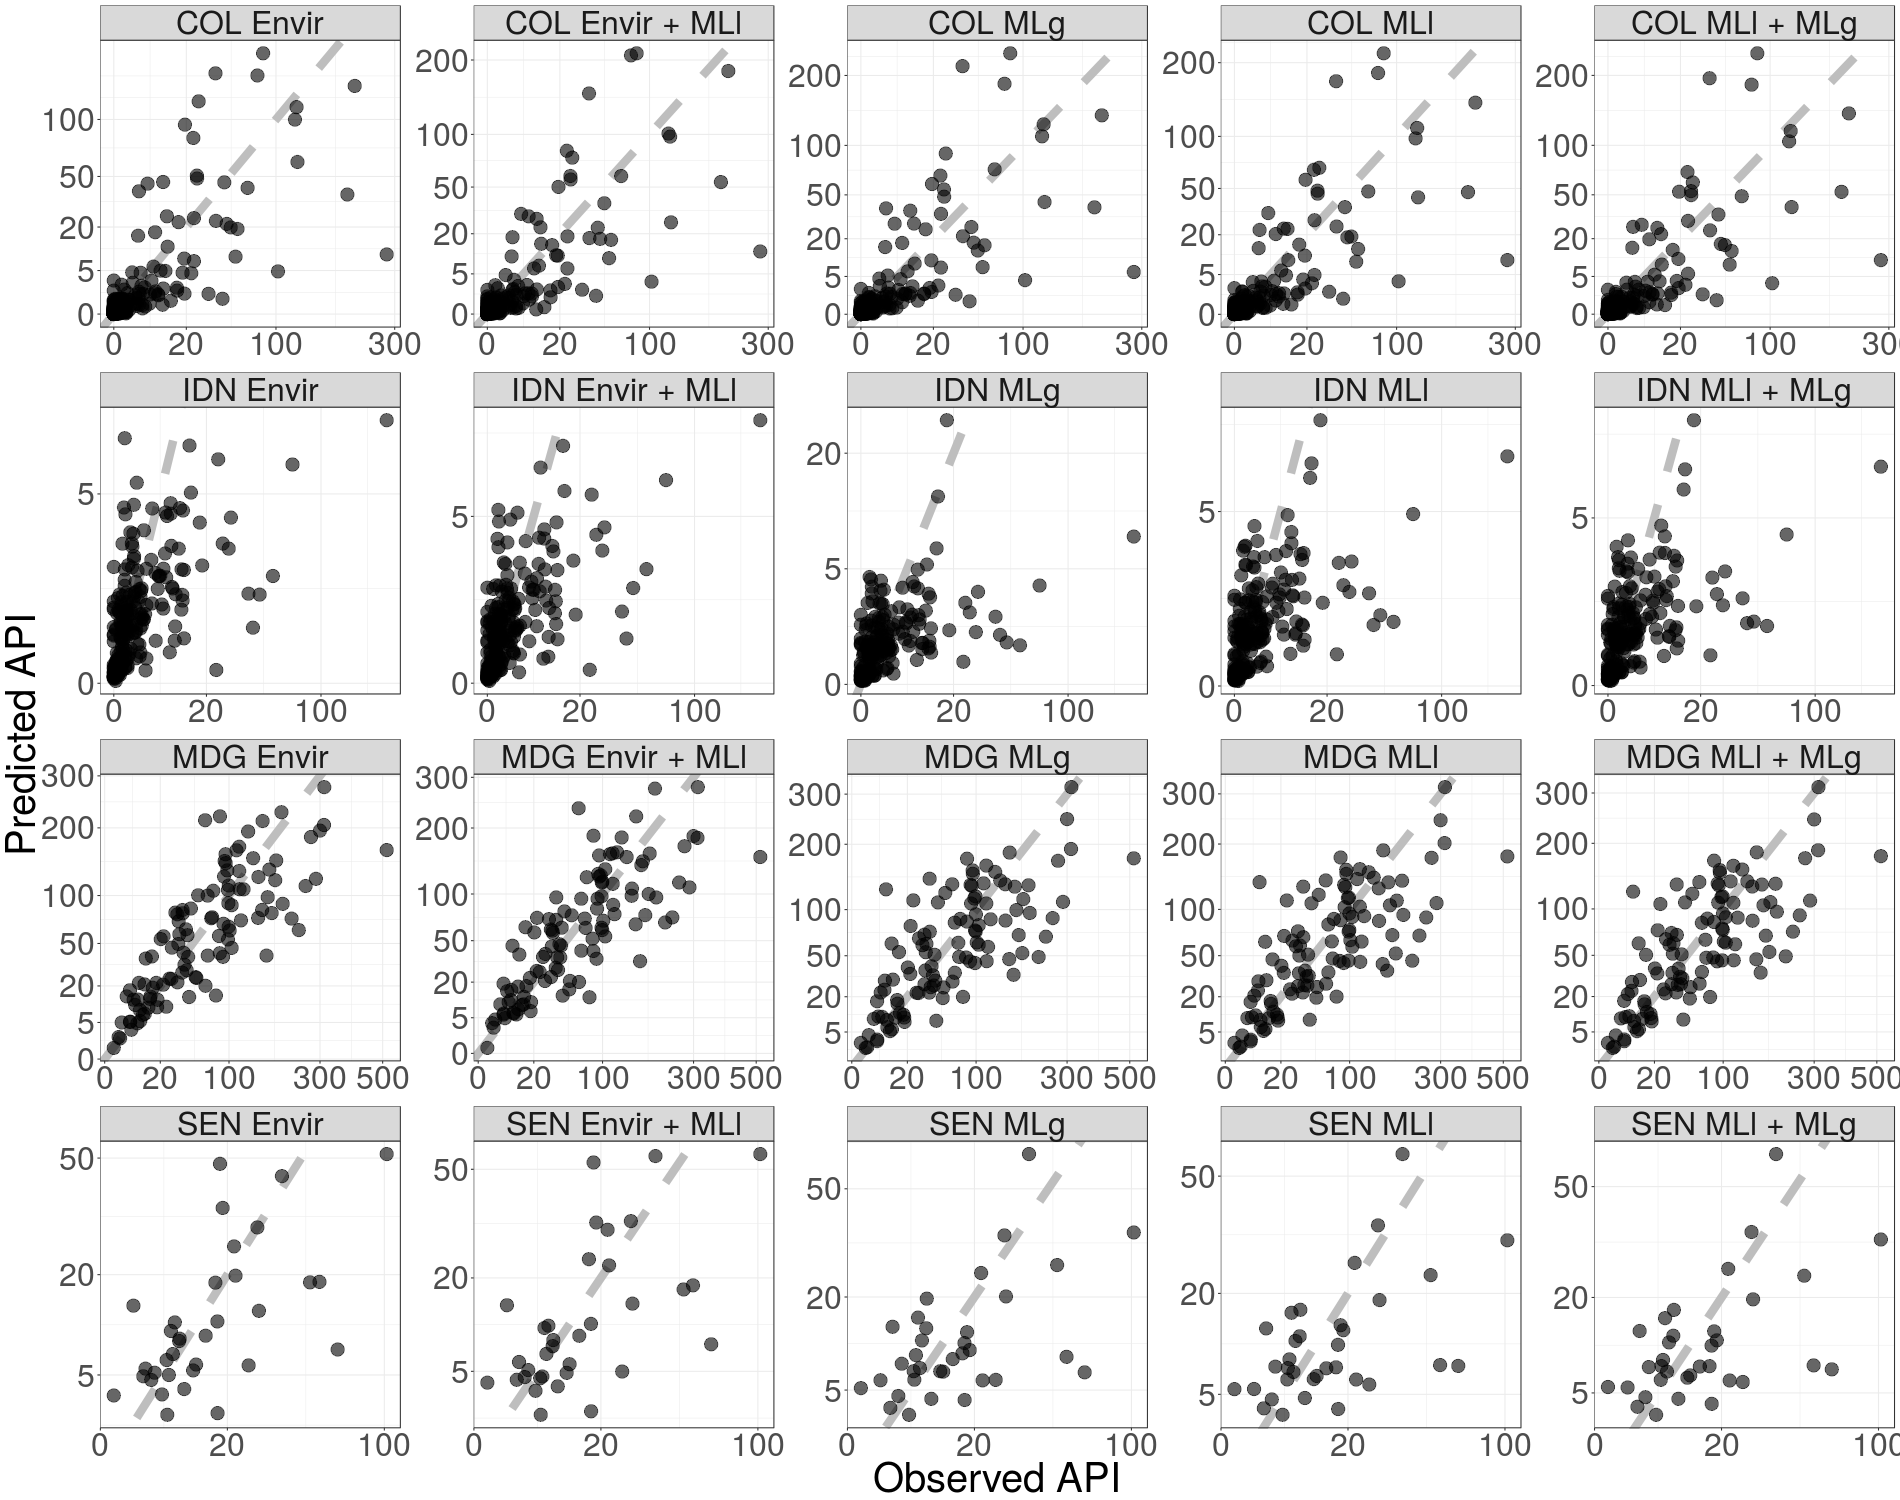
\includegraphics[width=\textwidth]{figs/cv1_scatter.png}
        \caption{Random cross-validation}
        \label{fig:cv1}
    \end{subfigure}
    \begin{subfigure}[b]{0.49\textwidth}
        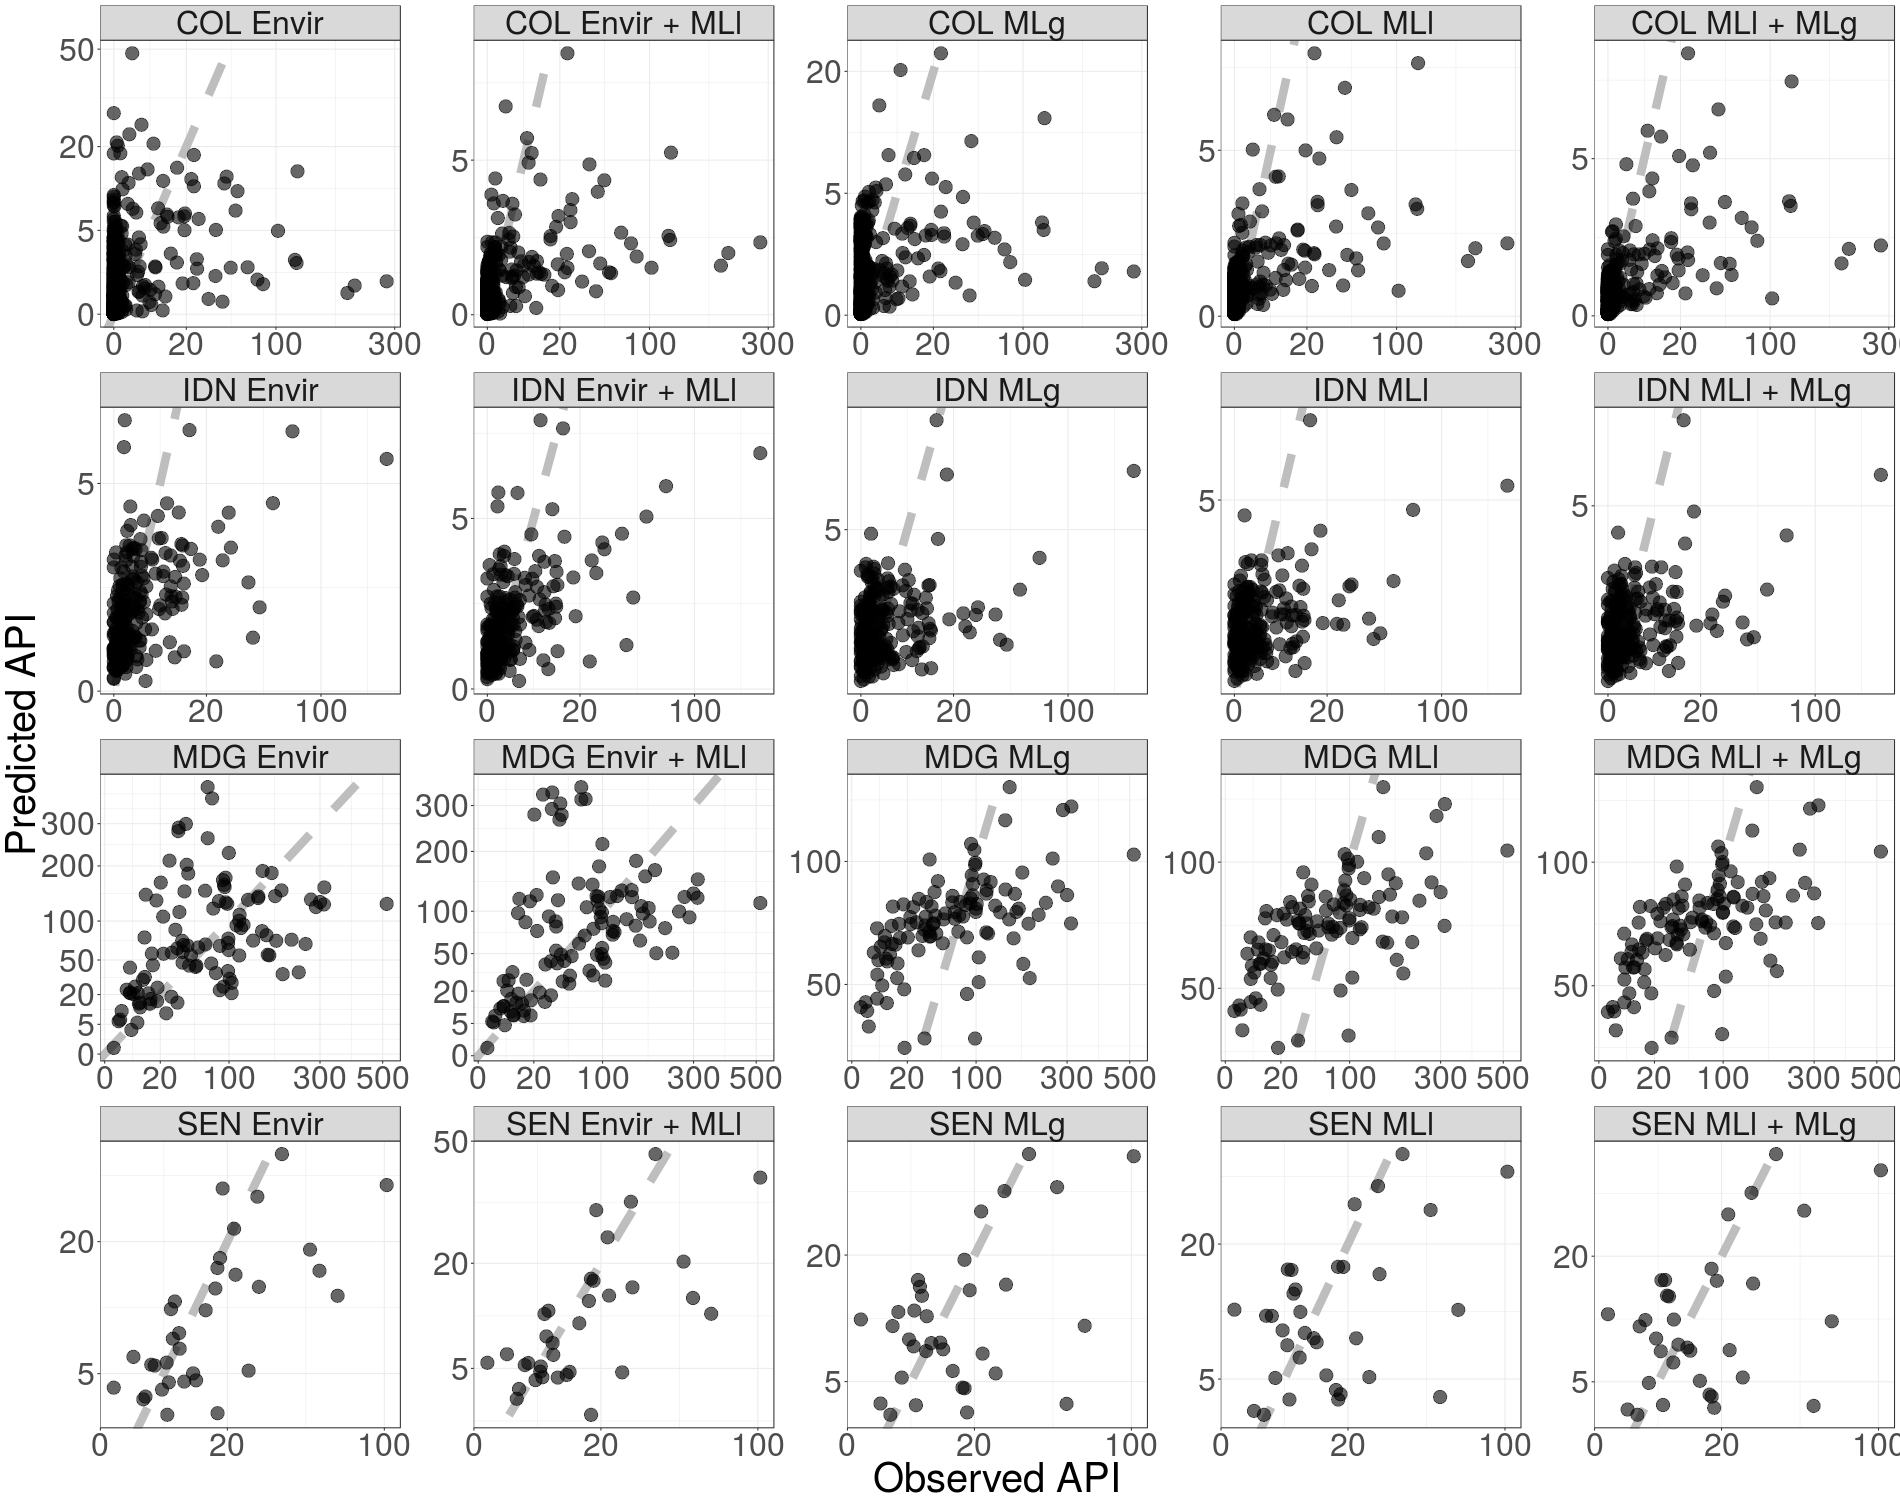
\includegraphics[width=\textwidth]{figs/cv2_scatter.png}
        \caption{Spatial cross-validation}
        \label{fig:cv1}
    \end{subfigure}
\caption{
  Observed data against predictions for cross-validation hold-out samples on a square root transformed scale.
  a) Seven-fold random cross-validation.
  b) Three-fold spatial cross-validation with folds indicated by colour.
}
\label{f:scatter}
\end{figure}



\begin{figure}
\centering
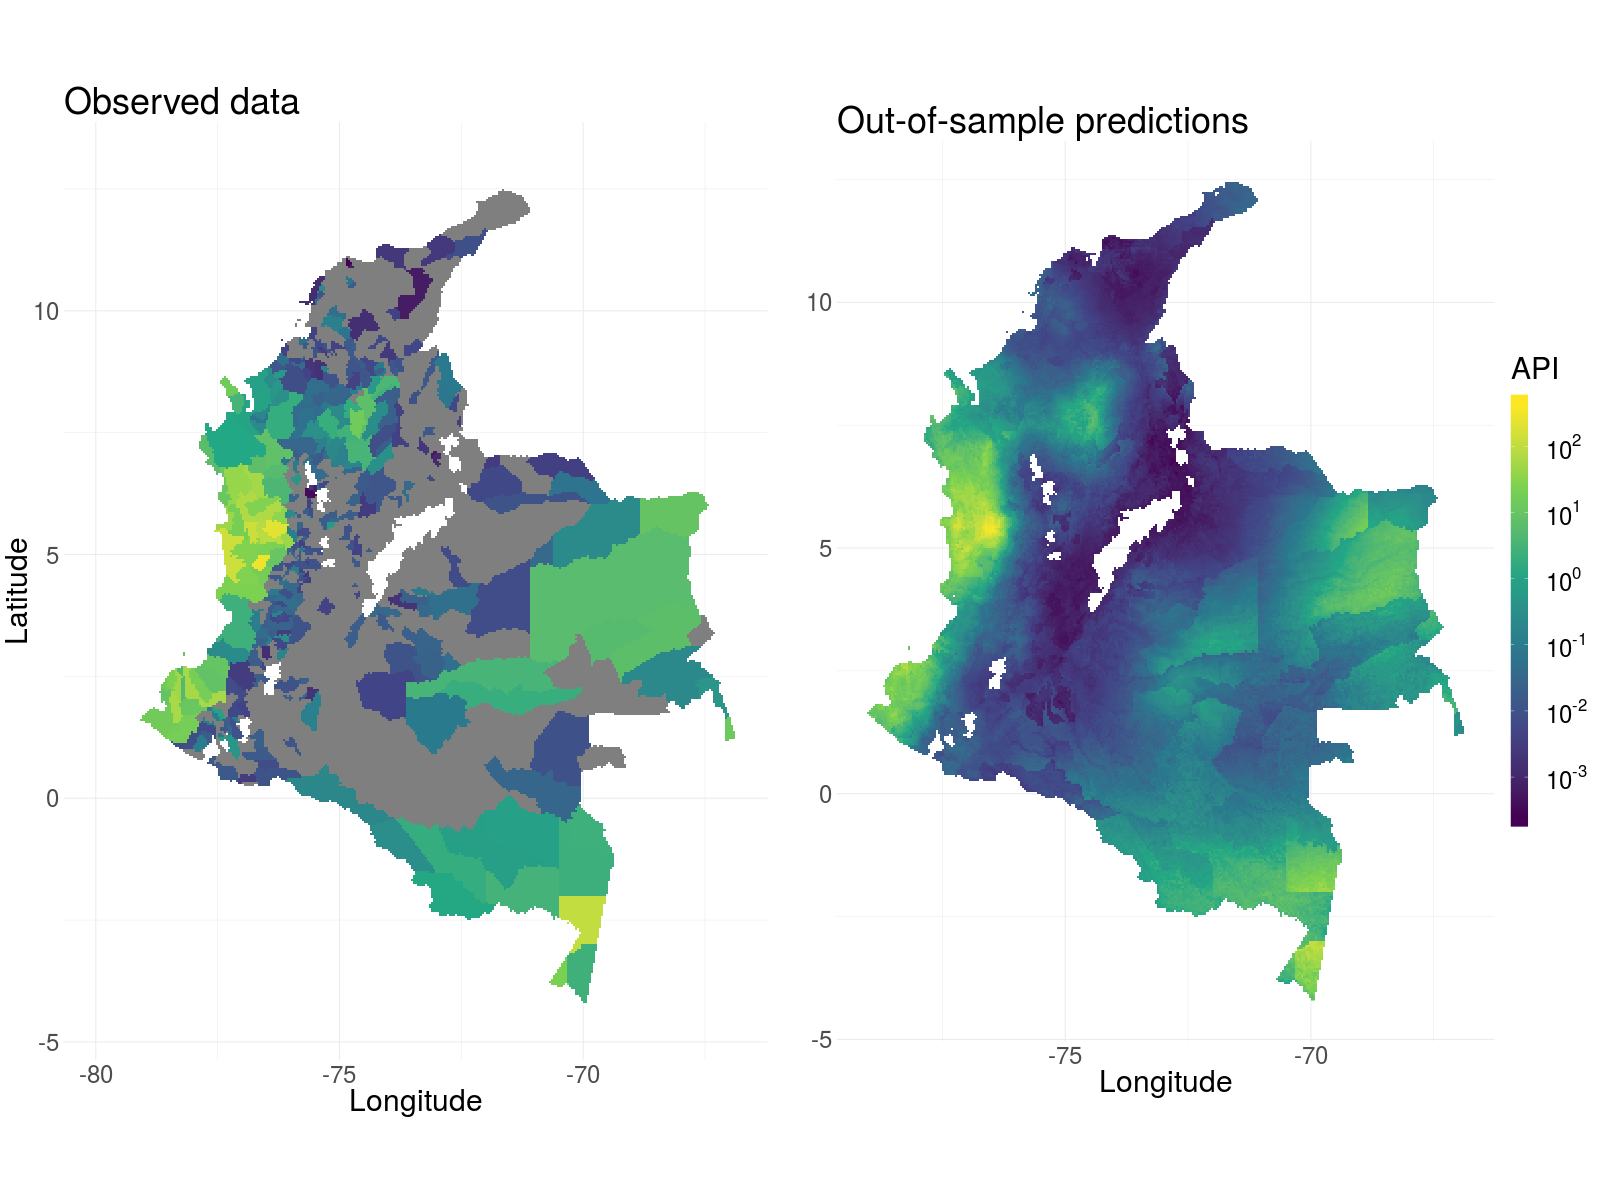
\includegraphics[trim={0 40mm 0 100mm}, width = 0.6\textwidth]{figs/col_obs_pred_map_ml.png} %\caption{Indonesia spatial crossvalidation} 
\caption{
  Left: Observed polygon data for Colombia. Grey indicates incidence of zero. Right: Out-of-sample predictions for the random cross-validation, machine learning model only model. For each cross-validation fold, predictions are made for the held out data. These predictions are all plotted which together covers the entire study area.
}
\label{randompredobspointfacet}
\end{figure}


\begin{table}
\caption{Pearson correlations between observed and predicted values. }
\centering
\begin{tabular}{lllll}
Cross-validation scheme & Country &  Covariates &  ML &  Covs + ML \\
\hline 
 Random &  Colombia &  0.45 &  \textbf{0.55} &  0.54 \\
 Random &  Madagascar &  0.70 &  \textbf{0.76} &  0.75 \\
 Spatial &  Colombia &  0.05 &  \textbf{0.18} &  0.10 \\
 Spatial &  Madagascar &  0.22 &  \textbf{0.63} &  0.61 
\end{tabular}
\label{t:results}
\end{table}



{\bf 5. Conclusions}




{\bf References}\\

\bibliography{Malaria} 
\bibliographystyle{plain}



\end{document}









